\documentclass[12pt,letterpaper]{article}

% --- Paquetes Requeridos ---
\usepackage[utf8]{inputenc}
\usepackage[spanish,es-tabla]{babel}
\usepackage[margin=2.5cm]{geometry}
\usepackage{graphicx}
\usepackage{float}
\usepackage{titlesec}
\usepackage{setspace}
\usepackage{hyperref}
\usepackage{booktabs}
\usepackage{caption}
\usepackage{enumitem}
\usepackage{listings}
\usepackage{xcolor}

% --- Configuración de Párrafo ---
\onehalfspacing
\setlength{\parindent}{0pt}
\setlength{\parskip}{1em}

% --- Rutas de búsqueda de imágenes ---
% Permite compilar tanto desde Documentos/Entregables/ como con todas las
% imágenes en una sola carpeta plana.
\graphicspath{{./}{../Evidencia/}{Evidencia/}{imagenes/}}

% --- Configuración de listings ---
\lstset{
    basicstyle=\ttfamily\footnotesize,
    breaklines=true,
    frame=single,
    captionpos=b,
    showstringspaces=false
}

% --- Inicio del Documento ---
\begin{document}

% --- PORTADA ---
\begin{titlepage}
    \centering

    {\Large \textbf{UNIVERSIDAD SANTO TOMÁS}} \\[1cm]

    {\Large \textbf{Sistema colaborativo de robots móviles para asistencia de orientación en entornos interiores con múltiples pisos}} \\[2cm]

    {\large \textbf{Realizado por:}} \\
    {\large Santiago Hernández Ávila} \\
    {\large Jonny Alejandro Mejía León} \\[1cm]

    \begin{figure}[H]
        \centering
        \includegraphics[width=0.6\textwidth]{Logos Uni.png}
        \label{Logo Universidad Santo Tomas y facultad de ingenieria electronica}
    \end{figure}

    \vfill

    {\large \textbf{Informe de Avance --- Semana 23}} \\
    {\large Fase 5: Integración del sistema y realización de pruebas --- Cierre de implementación: congelación del código, segundo vehículo y medición de los pasillos reales} \\[1.5cm]

    \textbf{Dirigido por:} \\
    Ing. Armando Mateus Rojas, Msc. \\
    Ing. Nestor Ivan Ospina, Msc. \\
    Ing. Oscar Mauricio Gélvez Lizarazo, Msc. \\[1.0cm]

    \vfill

    {\large GED (Grupo de Estudio y Desarrollo en Robótica)} \\
    {\large Facultad de Ingeniería Electrónica} \\
    {\large División de Ingenierías} \\
    {\large Bogotá, septiembre de 2026}
\end{titlepage}

% --- CONTENIDO ---

\section{Introducción}

El presente informe documenta el avance correspondiente a la \textbf{Semana 23} del cronograma de actividades (14 al 20 de septiembre de 2026), dentro de la \textbf{Fase 5 (Integración del sistema y realización de pruebas)}.

Es la semana de \textbf{cierre de implementación}: el 18 de septiembre se congeló el código con la etiqueta \texttt{v0.4-implementacion-congelada} (hito H7), y a partir de ahí no entra funcionalidad nueva. Llegó a esa fecha con \textbf{tres de los cuatro objetivos específicos cerrados}.

Tres resultados la definen. El \textbf{segundo vehículo} llegó el 14 de septiembre y la medida de red que llevaba un mes esperándolo se hizo ese mismo día; con ella cierran RF-15 y el riesgo R11, y el objetivo 2 se mueve por primera vez en cuatro semanas (Sección \ref{sec:red}). La \textbf{cancelación de misión} se verificó con corrida y control, y con ella el objetivo 3 cierra al 100~\% (Sección \ref{sec:rf29}). Y los \textbf{dos pasillos reales} quedaron medidos: ninguno da información de avance a la odometría láser, lo que cierra con evidencia la vía de construir el mapa del pasillo recorriéndolo y deja una sola ruta crítica (Sección \ref{sec:pisos}).

\section{Objetivos de la Semana}

El cronograma fija para esta semana el siguiente criterio de cierre:

\begin{quote}
\textit{El sistema corre de extremo a extremo en simulación y se ejecuta al menos una corrida física completa. Repositorio etiquetado.}
\end{quote}

Las actividades planificadas eran cuatro: verificación del funcionamiento general y corrección de fallas, ensayo en blanco del protocolo con los vehículos reales, congelación del código y emisión del informe de la Semana 22.

\textbf{El criterio se cumple en dos de sus tres partes.} La corrida física completa no ocurrió; se declara en la Sección \ref{sec:cronograma} como incumplida, sin reinterpretar el criterio.

\section{La cancelación de misión deja de ser inerte, y RF-29 se verifica corriendo}
\label{sec:rf29}

El botón de cancelar existía en la interfaz desde el 2 de septiembre y \textbf{no hacía nada}: \texttt{rclpy} rechaza por defecto toda cancelación si el servidor de acciones no registra un \texttt{cancel\_callback}, y nadie lo había registrado. El trabajo del fin de semana lo corrigió y, además, hace que una misión cancelada \textbf{devuelva el robot a la escalera de su piso} en lugar de dejarlo parado a mitad de pasillo.

Se enunció \textbf{RF-29} con cuatro condiciones y, en vez de dejarlo redactado, se corrió dos veces:

\begin{table}[H]
    \centering
    \small
    \caption{Las dos corridas de RF-29.}
    \label{tab:rf29}
    \begin{tabular}{@{}p{3.6cm}p{10.4cm}@{}}
        \toprule
        \textbf{Corrida} & \textbf{Resultado} \\ \midrule
        Cancelada & Marca \texttt{CANCELANDO}, cierre \texttt{FALLIDA}, robot a \textbf{0,121 m} de la escalera contra un criterio de 0,25 m \\ \addlinespace
        Control, sin cancelar & Ninguna marca de cancelación; cierre \texttt{COMPLETADA} \\ \bottomrule
    \end{tabular}
\end{table}

La cancelación se dispara \textbf{por distancia y no por tiempo} ---cuando \texttt{/odom} sitúa al robot a más de 8~m---, porque el robot nace a 1,4~m de la escalera: cancelar pronto satisfaría el criterio sin que el robot se hubiera movido.

\textbf{La corrida corrigió al requisito.} Se había escrito pidiendo que el registro trajera el motivo ``Cancelada por el usuario'', y el registro \textbf{nunca} lo trae: ese texto viaja en el resultado de la acción, que no se graba. Un criterio escrito con cuidado pedía comprobar un campo que no existe donde decía, y se corrigió antes de darlo por verificado.

\section{El segundo vehículo, R11 cerrado y RF-15 medido}
\label{sec:red}

El codirector entregó el segundo DeepRacer (\texttt{amss-jgm9}), y la latencia entre vehículos se midió el mismo día, con cotas fijadas \textbf{antes} de medir:

\begin{table}[H]
    \centering
    \small
    \caption{RF-15 medido entre los dos vehículos físicos, 14 de septiembre.}
    \label{tab:rf15}
    \begin{tabular}{@{}p{5.0cm}p{4.4cm}p{3.6cm}@{}}
        \toprule
        \textbf{Magnitud} & \textbf{Medido} & \textbf{Cota} \\ \midrule
        Mensajes & 600 de 600, 0~\% de pérdida & 0~\% \\ \addlinespace
        Ida y vuelta, mediana & \textbf{7,61 ms} & 100 ms \\ \addlinespace
        Ida y vuelta, p95 & \textbf{20,76 ms} & 250 ms \\ \bottomrule
    \end{tabular}
\end{table}

Con un margen de 13 veces en la mediana, \textbf{la red no limita} la publicación de estado a 2~Hz. Cierra RF-15, cierra R11 tras 31 días, y el objetivo 2 sube del 55 al 65~\%.

La sesión enseñó dos cosas que no estaban en el guion. \textbf{El cortafuegos tenía cortada la pareja de vehículos en los dos sentidos}: \texttt{ping} pasaba y el grafo de ROS salía vacío, de modo que RF-15 estuvo un mes en rojo por dos causas y solo una era el hardware. Y \textbf{la IP no identifica un vehículo entre sesiones}, porque el DHCP la cambia: los identificadores permanentes pasan a ser el nombre de máquina y la MAC.

\section{Los pasillos reales no dan información de avance}
\label{sec:pisos}

El vehículo no tiene encoders: su odometría la deduce \texttt{rf2o} comparando barridos consecutivos del LiDAR. En un pasillo recto y uniforme \textbf{el barrido siguiente es igual al anterior aunque el vehículo haya avanzado}, y la odometría devuelve cero. La herramienta \texttt{medir\_informacion\_avance.py} mide qué fracción de los rayos de un barrido informa del avance. Las referencias eran 13,8~\% en una caja cerrada simulada ---mapa aceptado--- y 6,8~\% en el pasillo simulado ---mapa rechazado---.

\begin{table}[H]
    \centering
    \small
    \caption{Información de avance de los dos pasillos reales.}
    \label{tab:pisos}
    \begin{tabular}{@{}p{6.0cm}p{6.0cm}@{}}
        \toprule
        \textbf{Entorno} & \textbf{Información de avance} \\ \midrule
        Pasillo real, piso 1 & \textbf{5,1~\%} \\ \addlinespace
        Pasillo real, piso 2 & \textbf{5,9~\%} ($n = 849$) \\ \bottomrule
    \end{tabular}
\end{table}

Para el piso 2 se escribió una \textbf{predicción antes de medir} ---entre 8 y 14~\%, porque tiene el doble de accidentes arquitectónicos--- y \textbf{quedó falsada}. La causa está en la Figura \ref{fig:decaimiento}: la información que aporta un hall \textbf{muere a los $\sim$6~m}, no a los 10--12~m de alcance del sensor que se habían supuesto. El umbral coincide con el que la Semana 22 había medido con otro instrumento.

\begin{figure}[H]
    \centering
    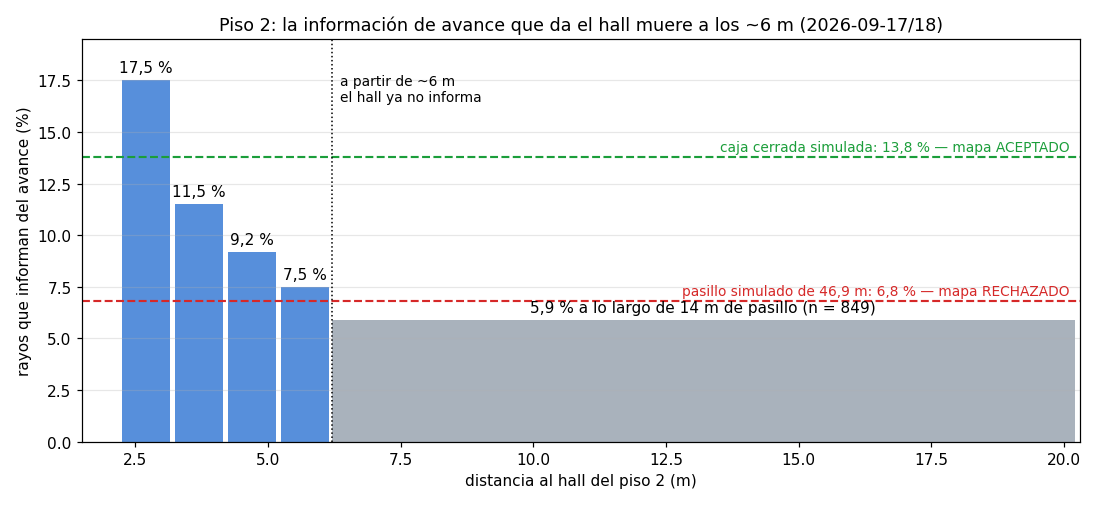
\includegraphics[width=0.95\textwidth]{S23_decaimiento_informacion_avance.png}
    \caption{Piso 2: la información de avance cae del 17,5~\% a 2,2~m del hall al 5,9~\% a partir de 6,2~m.}
    \label{fig:decaimiento}
\end{figure}

\textbf{Lo que esto no dice, y hay que escribirlo con el mismo peso:} no dice que el edificio no se pueda navegar. La campaña de evaluación en simulación corrió en esos mismos pasillos y dio \textbf{86,7~\% de éxito} con mapa conocido. Lo que el pasillo no soporta es \textbf{construir el mapa recorriéndolo}. De la corrida perdida del piso 2 salió además que \textbf{el LiDAR está montado girado 180$^\circ$}, de modo que su cuña ciega de 60$^\circ$ apunta hacia delante.

\section{La escala de tracción, medida sobre el vehículo}
\label{sec:rf14}

El 17 de septiembre se midió por primera vez la escala de \texttt{/cmd\_vel} sobre el carro, y trajo \textbf{dos defectos en lugar de uno}: además de que toda orden por debajo de 0,40~m/s sale como tracción cero, el nodo aplica un reescalado posterior que comprime los tres escalones a 0,4247 / 0,6242 / 0,7341. La dirección del vehículo nunca se había centrado, y se recalibró.

Y un \textbf{incidente de seguridad}: un solo comando de tracción \textbf{movió los dos vehículos}, porque comparten dominio de ROS y el tópico de servos no lleva espacio de nombres. Es el pendiente de espacios de nombres del objetivo 2 manifestándose como riesgo físico. Desde entonces, \textbf{en campo solo va encendido un vehículo}.

\section{Congelación, y el mapa de lo que queda}

El 18 de septiembre se congeló el código y se emitió \texttt{MAPA\_TRABAJO\_RESTANTE.md}, que acota en un solo documento todo lo que queda hasta la sustentación. Su lectura central: \textbf{hay una sola ruta crítica, y es publicar la transformada \texttt{odom} $\rightarrow$ \texttt{base\_link} en el vehículo real}. Los seis requisitos abiertos son todos de hardware.

\section{Otros avances de la semana}

\textbf{R14 queda cerrado} (16 de septiembre) con sus siete acciones, dos de ellas ejecutadas en contra de su enunciado y con la razón escrita. Al preparar la recomposición de los registros se comprobó que recomponer reescribía la procedencia en 44 de 44, así que \textbf{no se recompone ninguno}; de paso quedó probado que la cadena grabación $\rightarrow$ registro es reproducible, 44 de 44 sin mover un veredicto.

\textbf{El entregable versionado pasa a ser la fuente \texttt{.tex}}, no el PDF compilado en Overleaf.

\textbf{La secuencia de arranque queda escrita} en \texttt{GUIA\_ARRANQUE.md}: vivía repartida en la cabeza de dos personas, y ahora la puede ejecutar alguien que no estuvo.

\textbf{El capítulo de resultados de la campaña en simulación se adelantó de la Semana 24} (19 de septiembre). Encontró que los cuatro fallos son \textbf{un solo modo con nombre} ---Nav2 declara \texttt{SUCCEEDED} y \texttt{/odom} sitúa al vehículo entre 0,269 y 0,345~m de la meta--- y lo atribuye a la estimación de pose, entre 1,35 y 2,22 veces lo presupuestado. Deja escritas dos anotaciones incómodas: los criterios C1 y C2 no son independientes en ese modo, y tres misiones se corrieron dos veces sin motivo registrado.

\section{Aporte de la semana a los objetivos específicos}
\label{sec:aporte}

\subsection{Relación entre actividades y objetivos}

\begin{table}[H]
    \centering
    \small
    \caption{Trazabilidad entre las actividades ejecutadas y los objetivos específicos.}
    \label{tab:trazabilidad}
    \begin{tabular}{@{}p{4.4cm}cp{7.4cm}@{}}
        \toprule
        \textbf{Actividad} & \textbf{Objetivo} & \textbf{Contribución} \\ \midrule
        Cancelación de misión y RF-29 & OE3 & Último requisito del objetivo 3; lo cierra seis de seis \\ \addlinespace
        RF-15 con los dos vehículos & OE2 & Primer requisito de hardware verificado; cierra R11 \\ \addlinespace
        Información de avance de los dos pisos & OE2 & Cierra con evidencia la vía del mapa por SLAM en el pasillo \\ \addlinespace
        Escala de tracción sobre el vehículo & OE2 & Convierte RF-14 en una medida pendiente acotada \\ \addlinespace
        R14 y reproducibilidad de registros & OE4 & La campaña se regenera desde sus propios datos \\ \addlinespace
        Capítulo de resultados & OE4 & Nombra el modo de fallo y lo atribuye con cifras \\ \bottomrule
    \end{tabular}
\end{table}

\subsection{Estado de los objetivos específicos}

\begin{table}[H]
    \centering
    \small
    \caption{Avance por objetivo específico al cierre de la Semana 23.}
    \label{tab:objetivos}
    \begin{tabular}{@{}cp{2.8cm}p{4.2cm}p{4.6cm}@{}}
        \toprule
        \textbf{ID} & \textbf{Avance} & \textbf{Cubierto esta semana} & \textbf{Componente que lo mantiene detenido} \\ \midrule
        OE1 & 100~\% & --- & --- \\ \addlinespace
        OE2 & 55~\% $\rightarrow$ \textbf{65~\%} & RF-15 verificado; los dos pisos medidos & La cadena de odometría sobre el vehículo \\ \addlinespace
        OE3 & 90~\% $\rightarrow$ \textbf{100~\%} & RF-29 verificado & --- \\ \addlinespace
        OE4 & 85~\% & Resultados escritos; R14 cerrado & RF-27, la campaña física \\ \bottomrule
    \end{tabular}
\end{table}

El avance técnico agregado sin ponderar es del \textbf{87,5~\%} frente a un \textbf{71,9~\%} del calendario (semana 23 de 32). \textbf{Veintinueve de treinta y seis requisitos están verificados}. La tabla resumen del documento de requisitos decía 28, porque RF-15 no se había pasado a verificado en ella tras el 14 de septiembre; se corrigió el 25 de septiembre recontando fila por fila.

\textbf{Eso no es holgura.} Todo lo que falta es hardware, y no depende solo de horas de trabajo.

\section{Estado del cronograma y trabajo previsto}
\label{sec:cronograma}

\subsection{Cumplimiento del criterio de cierre}

\begin{table}[H]
    \centering
    \small
    \caption{Criterio de cierre de la Semana 23 y su evidencia.}
    \label{tab:cierre}
    \begin{tabular}{@{}p{5.6cm}cp{6.0cm}@{}}
        \toprule
        \textbf{Exigencia del criterio} & \textbf{Estado} & \textbf{Evidencia} \\ \midrule
        El sistema corre de extremo a extremo en simulación & Cumplido & Corridas de RF-29 el 14 de septiembre; misión desde teléfono de la Semana 22 \\ \addlinespace
        Se ejecuta al menos una corrida física completa & \textbf{No cumplido} & La primera navegación sobre el vehículo ocurre el 24 de septiembre, en la Semana 24 \\ \addlinespace
        Repositorio etiquetado & Cumplido & \texttt{v0.4-implementacion-congelada}, 18 de septiembre \\ \bottomrule
    \end{tabular}
\end{table}

\subsection{Lo planificado frente a lo hecho}

De las cuatro actividades previstas se ejecutaron \textbf{tres}: verificación y corrección de fallas, congelación del código y emisión del informe anterior. \textbf{El ensayo en blanco del protocolo con los vehículos reales no se ejecutó}, porque la cadena de odometría del vehículo no existía todavía.

Surgieron sin planificar la llegada del segundo vehículo, la medición de los dos pisos, la escala de tracción en campo y el capítulo de resultados. Se declaran como tales.

\subsection{Trabajo previsto para la Semana 24}

Resolver el GO/NO-GO de la demostración física, publicar la odometría en el vehículo ---la ruta crítica---, consolidar el conjunto de datos de la campaña y emitir este informe.

\section{Conclusiones de la Semana}

\begin{enumerate}[leftmargin=*]
    \item \textbf{La implementación está congelada con tres de cuatro objetivos cerrados}, y el que falta es el de la plataforma física.
    \item \textbf{El segundo vehículo cerró un requisito el día que llegó}, y enseñó que la mitad de su bloqueo no era hardware sino un cortafuegos.
    \item \textbf{El objetivo 3 queda completo}, y su último requisito se corrigió al correrlo, no al escribirlo.
    \item \textbf{Los pasillos reales no dan información de avance}, medido en los dos pisos y con una predicción falsada por el camino. Se cierra con evidencia una vía y queda una sola ruta crítica.
    \item \textbf{La corrida física completa que pedía el criterio no ocurrió.} Se declara incumplida en lugar de reinterpretar el criterio.
\end{enumerate}

\section{Anexos}

Las cifras de este informe proceden de los registros y documentos de evidencia versionados en el repositorio del proyecto. Existe una versión en Markdown de este mismo informe, \texttt{Entregable\_semana\_23.md}, legible directamente en el repositorio.

\begin{thebibliography}{99}

\bibitem{rf29}
S. Hernández Ávila y J. A. Mejía León,
``RF-29: corrida cancelada y corrida de control,''
Repositorio del proyecto, \texttt{Documentos/Evidencia/registros/S23\_RF29\_cancelada.json} y \texttt{S23\_RF29\_control.json}, septiembre de 2026.

\bibitem{rf15}
S. Hernández Ávila y J. A. Mejía León,
``RF-15 medido entre los dos vehículos físicos,''
Repositorio del proyecto, \texttt{Documentos/Evidencia/registros/S23\_RF15\_carroA\_carroB.json}, septiembre de 2026.

\bibitem{pisos}
S. Hernández Ávila,
``Información de avance del pasillo real, pisos 1 y 2,''
Repositorio del proyecto, \texttt{Documentos/Evidencia/S23\_informacion\_avance\_piso1.md} y \texttt{S23\_informacion\_avance\_piso2.md}, septiembre de 2026.

\bibitem{rf14}
S. Hernández Ávila,
``RF-14: la escala de tracción medida sobre el vehículo,''
Repositorio del proyecto, \texttt{Documentos/Evidencia/S23\_campo\_traccion\_RF14.md}, septiembre de 2026.

\bibitem{reproducibilidad}
S. Hernández Ávila,
``Reproducibilidad de los registros de la campaña,''
Repositorio del proyecto, \texttt{Documentos/Evidencia/S23\_reproducibilidad\_de\_los\_registros.md}, septiembre de 2026.

\bibitem{mapa}
S. Hernández Ávila y J. A. Mejía León,
``Mapa del trabajo restante y plan hasta la sustentación,''
Repositorio del proyecto, \texttt{Documentos/MAPA\_TRABAJO\_RESTANTE.md}, septiembre de 2026.

\bibitem{resultados}
S. Hernández Ávila y J. A. Mejía León,
``Resultados de la campaña de evaluación en simulación (OE4),''
Repositorio del proyecto, \texttt{Documentos/RESULTADOS\_OE4\_SIMULACION.md}, septiembre de 2026.

\end{thebibliography}

\end{document}
